\section{Hubo2 Plus}
Hubo2 Plus, Hubo for short, is a 130 $cm$ (4' 3'') tall, 42 $kg$ (93 $lb$) full-size humanoid robot.  
It was designed and constructed by Prof Jun-Ho Oh and the Hubo Lab at the Korean Advanced Institute of Science and Technology\cite{hubo-first}.
Hubo has 2 arms, 2 legs and a head, making it anthropomorphic to a human.  
It boasts 38 degrees of freedom (DOF) consisting of 6x in each leg, 6x in each arm, 5x in each hand, 3x in the neck, and 1x in the waist.
All joints with the exception of the fingers are high gain PD position controlled.
The fingers are PWM controlled.
It has a three axis force torque (FT) sensor on leg between the end of the ankle and the foot and on the arm where it connects to the hand.
Additionally it has accelerometers on each foot and a six axis inertial measurement unit (IMU) slightly below it's weight (approximately the centre of mass).
The reference commands for all of the joints are sent from the primary control computer (x86) to the individual motor controllers via two Controller Area Network (CAN) buses.
There are currently eight Hubo's functioning in the United States as of December 2012.
Four reside at Drexel University and one at Georgia Tech, Perdue, Ohio State and MIT.
Jaemi Hubo is the oldest of the Hubos in America and has been at the Drexel Autonomous Systems Lab\footnote{Drexel Autonomous Systems Lab: http://dasl.mem.drexel.edu/} (DASL) since 2008\cite{jaemiHuboSRM}.
Fig.~\ref{fig:hubo} shows the major dimensions of Hubo.

\begin{figure}[thpb]
  \centering
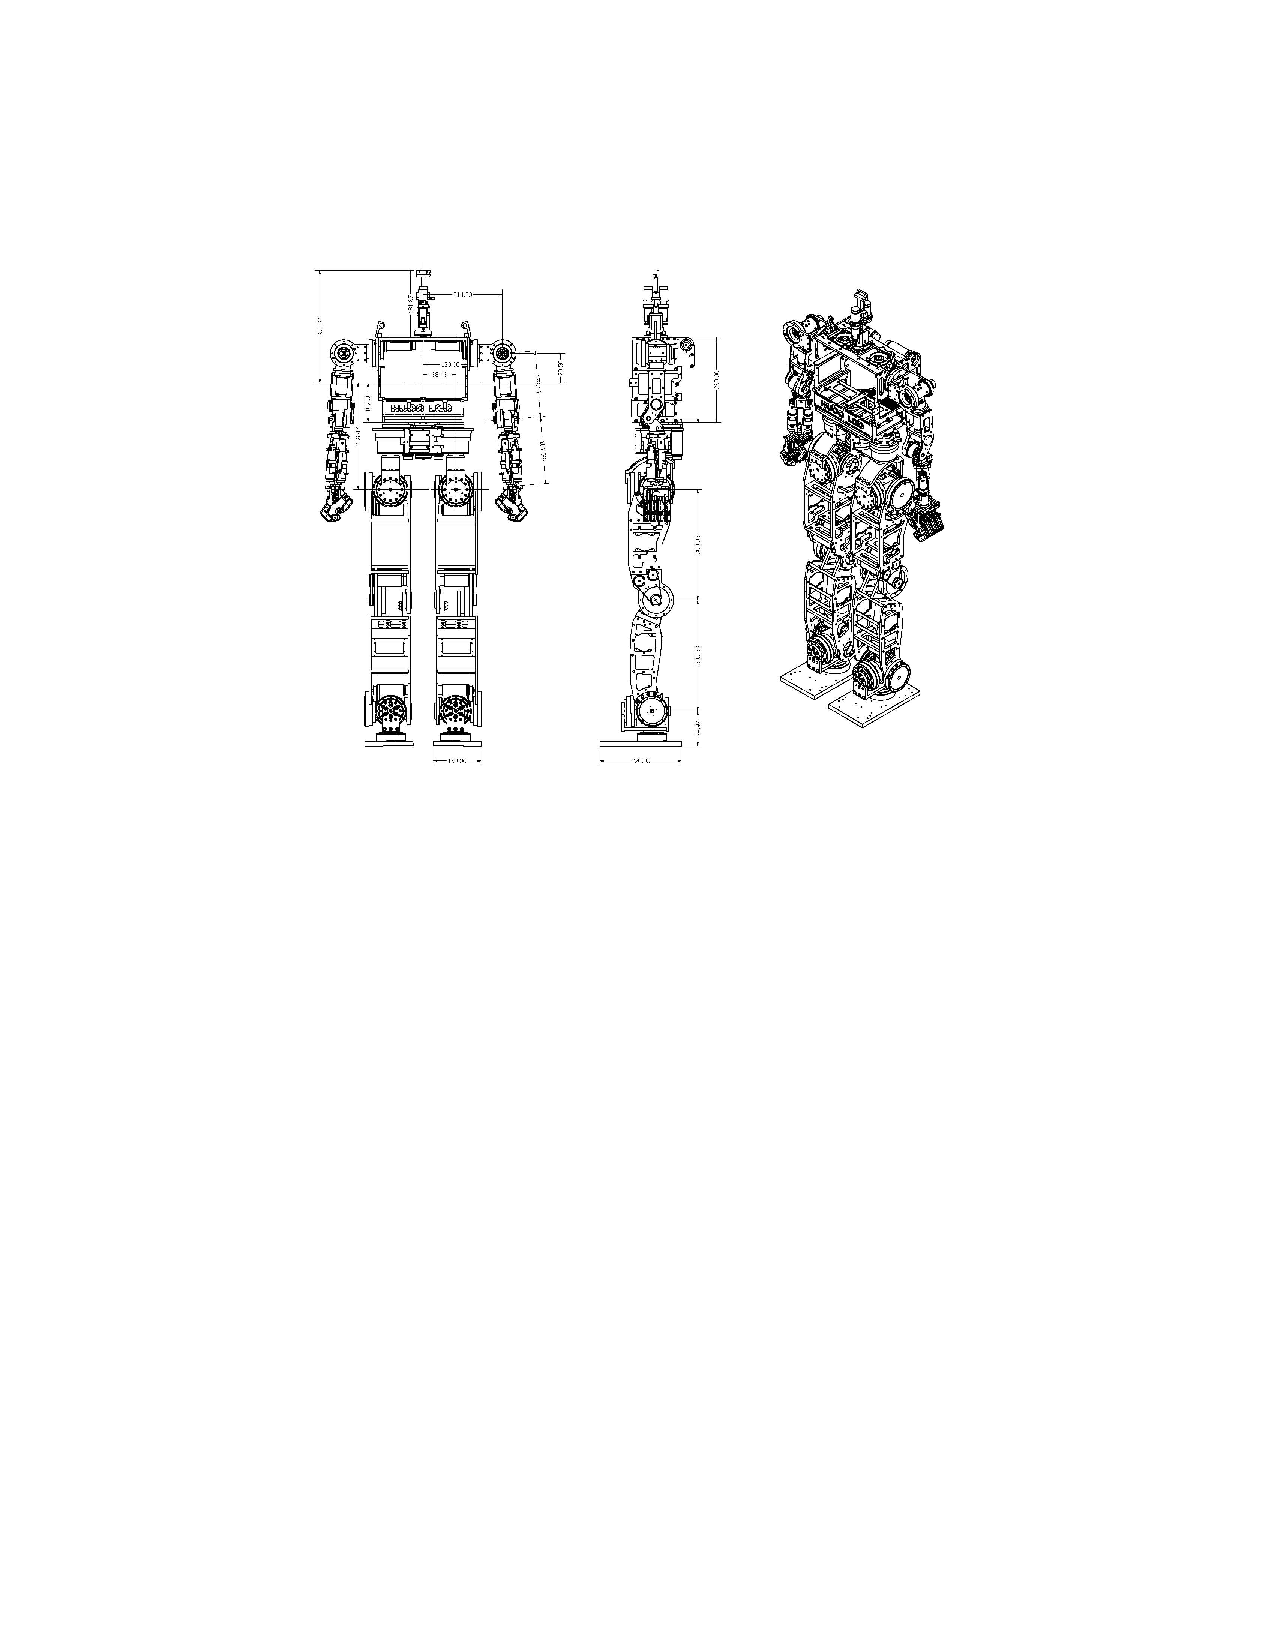
\includegraphics[width=1.0\columnwidth]{./pix/huboSkel.pdf}
  \caption{Hubo2 platform: 130 $cm$ tall full-size humanoid robot weighing 37 $kg$.  It has 38 DOF consisting of 6x in each leg, 6x in each arm, 5x in each hand, 1x in the waist, and 3x in the neck.}
  \label{fig:hubo}
\end{figure}



